
\documentclass{article}
\usepackage{verbatim}
\usepackage{amssymb}
\usepackage{amsmath}
\usepackage{mdwlist}
\usepackage{graphicx}

\title{Explorer scenario specification for Bham meeting}
\date{\today}
\author{CoSy Explorer group, Hendrik}


\begin{document}
\maketitle

\section{Script -- level 1}
\subsection{Scenario 1}
\label{scen1}
\textit{Scenario 1, cf. Specs}

\begin{enumerate}
\item Robot is idling in the corridor. 
\item User approaches the robot.
\item \label{lvl1:user_asks_1}
	User asks robot: ``Could you go and find the Borland book, please?''
\item \label{lvl1:rob_answs_1}
  	Robot says: ``I will go and look for it in a library where books are normally found.''
\item \label{lvl1:user_answs_2}
	User answers: ``Ok.''
\item \label{lvl1:rob_goes_lib}
	Robot moves to the library.
\item \label{lvl1:look_for_book}
	Robot looks for the book.


\emph{deviation from original scenario script!}
\item \label{lvl1:not_find_book}
	Robot does not find it.
\item \label{lvl1:look_for_person}
	Robot looks for a person (to ask).
\item \label{lvl1:}
	Robot asks: ``Do you know where the Borland book is?''
\item 
	Person answers: ``I believe it is in GJ's office.''
\item
	Robot says: ``Okay.'' and takes off to GJ's office.
	
\item 
	Robot enters GJ's office and finds the Borland book.
\item
	Robot goes back to the user.
\item
	Robot finds user and says ``The book is in GJ's office near the Starbucks mug.''
	
\end{enumerate}


%\begin{figure}[ht]
%\centering
%\includegraphics[width=\linewidth]{example1_msc.png}
%\caption{
%  Some simple msc-graph can be generated to clarify interaction
%  between things in the the scenario. Use the
%  \texttt{../gen\_msc.sh}-script to generate pngs from all
%  msc-files. mscgen is documented here:
%  \texttt{http://www.mcternan.me.uk/mscgen/}. It's VERY simple}
%\label{fig:lvl1}
%\end{figure}


\section{Script -- level 2}
\textit{
  The level 1 script describes what can obviously be seen when the
  robot is interacting, for example in a video uptake of the
  scenario. The next level is to describe, without any technical
  detail, what activities take place within the robot during this
  interaction. }



\begin{enumerate}
\item \label{lvl2:1}
	The robot is idle (with some initial info).
	\begin{enumerate}
	\item Robot is in Hendrik's office and so is Hendrik.
	\item It has a map of the environment with H's office, 
			GJ's office, a corridor, and the library.
	\item Robot has ontological knowledge that books are 
			in libraries and can recognize the Borland book.
	\end{enumerate}
\item \label{lvl2:2} 
	User comes up to the robot.
	\begin{enumerate}
	\item Robot detects a person approaching
	\item Robot looks at the ``user''
	\item 	
	\end{enumerate}

\item \label{lvl2:3} 
	User asks robot...
	\begin{enumerate}
	\item Utterance gets interpreted and translated into a command
	\item Motive generated on basis of command
	\item ``BorlandBook'' is on the binder\footnote{could be represented
		as mental note tag; maybe associated with a probability}
	\item Robot does inference and planning
		\begin{itemize}
		\item plan: where is location of BorlandBook
		\item result: does not know location of this instance
		\item infer: type of BorlandBook is book; books are usually found in libraries
		\item plan: path to library
		
		\end{itemize}
	\end{enumerate}

\item \label{lvl2:4} 
	Robot gives feedback (answer) based on generated plan
	\begin{enumerate}
	\item Robot plans a response
	\item Robot utters the response
	\end{enumerate}

\item \label{lvl2:5} 
	Users confirms (``Ok.'')
	\begin{enumerate}
	\item Robot interprets utterance as a confirmation and 
		allows the plan to be executed.
	\end{enumerate}
	
\item \label{lvl2:6} 
	Robot moves to library
	\begin{enumerate}
	\item Robot moves through a door into corridor, follows it and enters library through a door
	\item (Robot verifies that it is the library)
	\end{enumerate}

\item \label{vis_search_lib} \label{lvl2:7} Robot looks for book
	\begin{enumerate}
	\item Robot creates a plan to search the room for finding the 
		book\footnote{this might correspond to planning of visual operators done by Mohan;
			KTH should clarify potential overlap or contradictions with Mohan}
	\item Executes the visual search plan
	\end{enumerate}

\item \label{vis_search_lib_fail} \label{lvl2:8} Robot does not find it
	\begin{enumerate}
	\item Plan ends; no book found\footnote{need to represent fact that we have not
		succeeded finding the book instance}
	\item (Adds explicit negation ``book is not in library'' to planning 
		state)\footnote{probabilities of typical knowledge could be linked to threshold
		function -- problem: probabilities will be very low if there are many rooms.}
	\end{enumerate}
	
\item \label{lvl2:9}
	Robot looks for person to ask
	\begin{enumerate}
	\item Visual search (plan) failure triggers re-planning
	\item New plan involves finding and asking a person
	\item looks for a person and finds one
	\item drives up to the person
	\end{enumerate}
	
\item \label{lvl2:10} 
	Robot asks person ``Do you know where the Borland book is?''
	\begin{enumerate}
	\item Plans a dialogue and utters question
	\end{enumerate}

\item Persons answers: ``I believe it is in GJ's office.''
	\begin{enumerate}
	\item Robot interprets that as an answer to its question
	\item resolves ``it'' to BorlandBook
	\item Robot extracts the position info
	\item (BorlandBook + pos info represented on binder (updated) with modality)
	\end{enumerate}

\item Robot says ``Okay.'' and takes off to GJ's office
	\begin{enumerate}
	\item planner plans moveTo(GJ's office) action
	\item starts moving to GJ's office
	\end{enumerate}
	
\item Robot enters GJ's office and finds BB.
	\begin{enumerate}
	\item see \ref{vis_search_lib} and \ref{vis_search_lib_fail}, but now finding it
	\item adds book position
	\end{enumerate}

\item Robot goes back to user
	\begin{enumerate}
	\item continues execution of original plan, which involves
		\begin{itemize}
		\item assumes user in same place
		\item moves back there
		\end{itemize}
	\end{enumerate}

\item Robot finds user and says ``book is in GJ's office near the mug...''
	\begin{enumerate}
	\item looks for a person and assumes it is the user
	\item robot verbalizes opsition of the book
	\end{enumerate}

\end{enumerate}

\section{List of subarchitectures}

\subsection{motivator}
look for people to interact with 
(passively! get ready for interaction, 
pay attention to people; replace Y2 ``wake up function'')

listen for event structures on the binder: ``find'' can be transormed
into a planning goal

\subsection{vision.sa}


\subsection{navigation.sa}
SLAM, graph building, people detection (laser-based, ?vision?)

KTH; overall responsible: Patric

\subsection{planner}
get goal from MotiveGenerator and Handler

\subsection{binder}

\subsection{comsys}

\subsection{coma.sa}


\subsection{spatial}
same as in PlayMate!
near, left of, right of


\section{Subarchitecture Level}
\textit{
  Describe for each step in the detailed lvl2 script what the involved
  subarchitectures are and how they are involved.}
  
\begin{figure}[bth]
\centering
	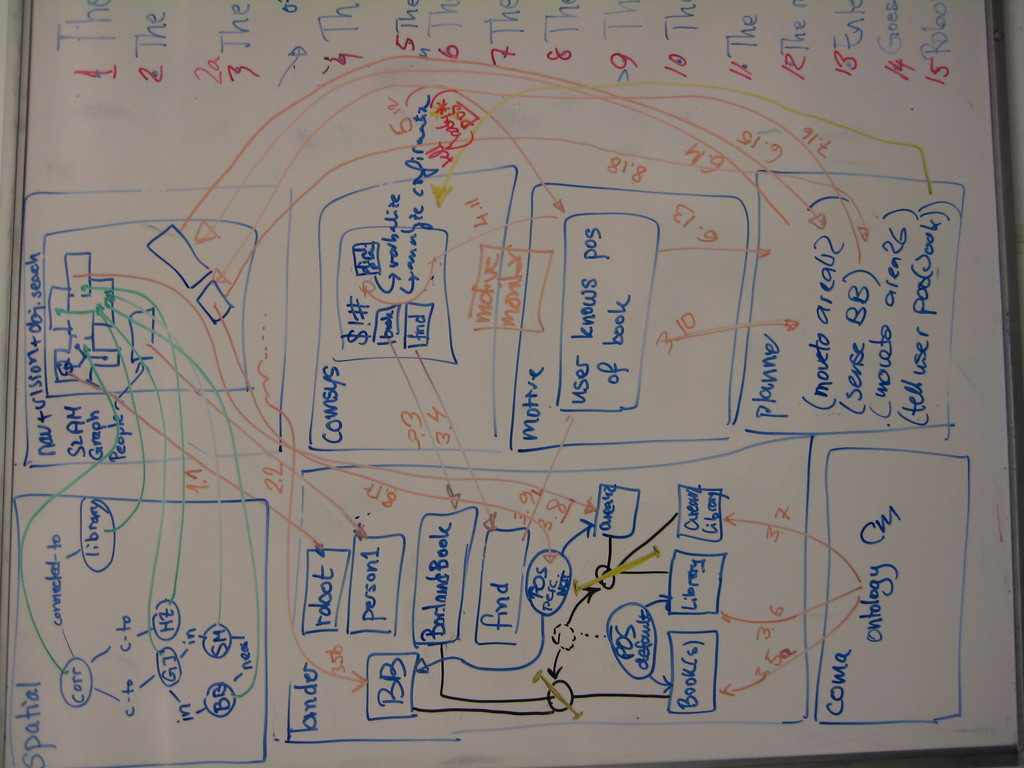
\includegraphics[angle=-90,width=\linewidth]{ex-img_0051.jpg}
	\caption{Final drawing of SA interaction: Orange arrows denote stepwise
	processing. The first number is the index of the level 2 description, the second
	number is an incremental global index over all processes.} 
\label{fig:subarch_interaction}
\end{figure}

  
\subsection{\ref{lvl2:1}} smth in the binder called ``me'' (ie the robot),
	which has a position (by ?nav.sa?); cf. Fig. \ref{fig:nav_orig}
  
\subsection{\ref{lvl2:2}} User detection triggered by laser and 
	verified by vision
	person represented on the binder (put there by the person detector/tracker), cf. Fig. \ref{fig:nav_orig}
	open question: how to trigger look at user

\begin{figure}[bth]
\centering
	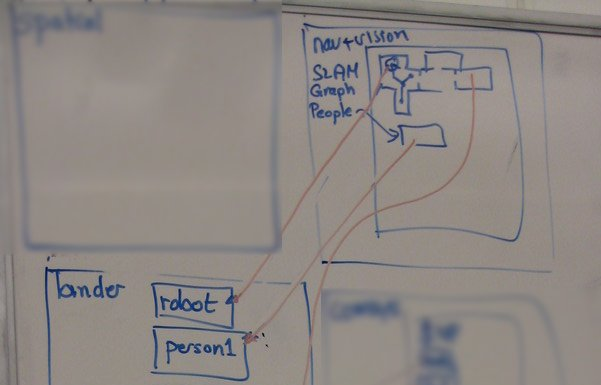
\includegraphics[width=\linewidth]{explorer_1.jpg}
	\caption{Original state of the binder: nav.sa represents the robot and the user on the binder.
	Not shown is the representation of the robot's and the user's current (topological) positions.} 
\label{fig:nav_orig}
\end{figure}


\subsection{\ref{lvl2:3}} User asks robot...
	utterance parsed by comsys; produces a logical form that expresses that there
	is a request for finding the object
	proxy for ``you'' = addressee/hearer resolved via binder to robot proxy;
	proxy for ``BorlandBook'' by comsys;
	proxy for event structure ``find the book'' by comsys
	behind the scenes: transform that into knowledge goal by MotiveGenerator
	generate goal for planner: user\_knows(pos(book))
	This is shown in Fig. \ref{fig:comsys_plan}.
	
	
	coma.sa notices mention of "borland book"; since it does not know
	concrete information, it decides to provide default knowledge:
	coma.sa creates a proxy ``Book" (or ``Books'' if plural handling works!)
	and a proxy ``Library'' and links them with a ``position'' relation proxy.
	This relation proxy is tagged as ``default''.
	Coma.sa furthermore provides proxies for all libraries that it knows about,
	in this case a single proxy for ``area 42''.
	Nav.sa notices that and provides a proxy for its internal ``area 42''
	Now comes the binder: 
	``BorlandBook'' and ``Book'' get bound to the same union (u1)
	``Library'' (abstract) and ``Library / area 42'' (concrete) from coma.sa get bound (u2);
	``area 42'' from nav.sa ends up in the same union (u2)!
	Those unions (u1 and u2) will also be linked by the ``position'' (default) relation.
	This is shown in Fig. \ref{fig:coma_default}.



	Planner works out a plan (cf. Fig. \ref{fig:planner})
	(moveto area42)
	(sense BB)
	(moveto area26)
	(tell user pos(book))

\begin{figure}[bth]
\centering
	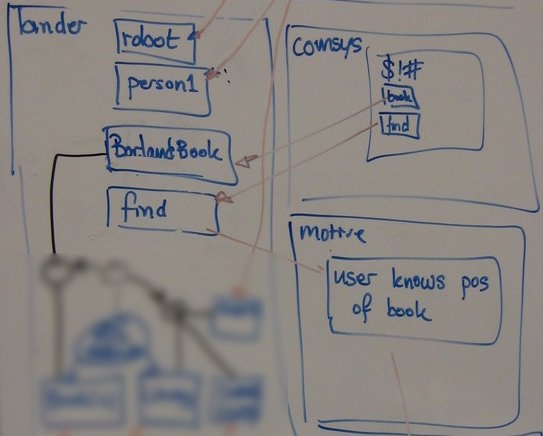
\includegraphics[width=\linewidth]{explorer_2.jpg}
	\caption{add caption!} 
\label{fig:comsys_plan}
\end{figure}

\begin{figure}[bth]
\centering
	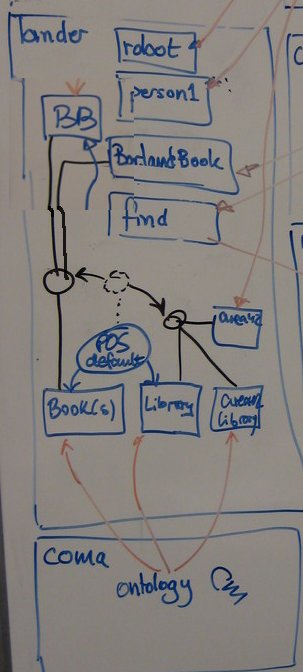
\includegraphics[width=\linewidth]{explorer_3.jpg}
	\caption{add caption!} 
\label{fig:coma_default}
\end{figure}

\begin{figure}[bth]
\centering
	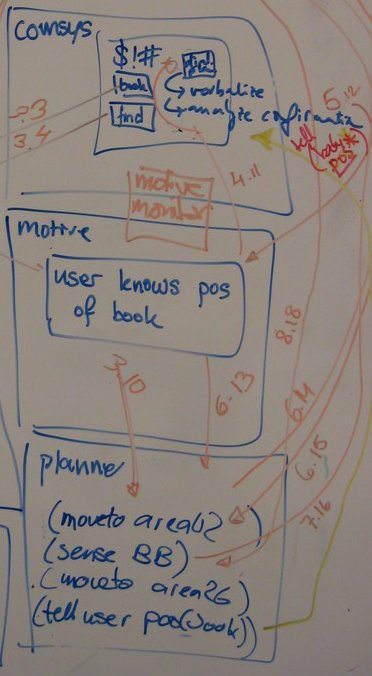
\includegraphics[width=\linewidth]{explorer_4.jpg}
	\caption{add caption!} 
\label{fig:planner}
\end{figure}



\subsection{\ref{lvl1:rob_answs_1}} Planner can come up with a satisfiable plan. Planner can provide
	MotiveHandler tells comsys about the outcome of planning to give verbal feedback
	-- MotiveMonitor between motive.sa and comsys.sa
	\begin{enumerate}
	\item satisfiability (``yes'')
	\item goal state (``will go to Y'')
	\item based on instance or default knowledge (``X is in Y'' vs ``X'es are typically found in Y's'')
	\end{enumerate}

\subsection{\ref{lvl2:5}} Comsys interprets confirmation


\subsection{\ref{lvl2:6}} MotiveHandler/monitor notices acknowledgement by comsys
	MotiveHandler triggers execution of the plan by the planner
	Planner passes (moveto area42) action to nav.sa, which executes it (mark in struct ``ACK")
	-- and succeeds (mark in struct ``DONE")

\subsection{\ref{lvl2:7}} Planner sends (sense BB) action to nav.sa, which runs 
	visual search planning + execution (mark in struct ``ACK")
	
\subsection{\ref{lvl2:8}} Visual search fails; 
	nav.sa adds NEGATED ``position'' relation between BB and area42;
	BB will be removed from the ``Book(s)'' (abstract) union;
	``area42/lib'' (concrete, coma.sa) and area42 (concrete, nav.sa) will be removed from the ``Library'' (abstract) union;
	\footnote{coma.sa could take the fact that BB is not in the Book(s) union anymore as an
		indication to remove the default proxies -- because those were provided because of
		/ triggered by BB}

\subsection{\ref{lvl2:9}} Robot needs to look for person to ask
	should people tracking run constantly throughout the experiment? Or only on-demand?
	
	If the motive is ``look for person and ask'', people tracker can
	provide knowledge about persons to the binder.
	
	The planner could also have an action ``find person'' that will
	trigger a specific behavior by the people recognition.
	
	This could also be handled by ``information request'' / ``clarification
	request'': create a proxy ``Person'' w/o any additional information and
	request position information.


	go to person = goto(person)
	
\subsection{\ref{lvl2:10}}
	Comsys plans a dialogue to fulfill askPersonAboutBook command.
	


\subsection{\ref{lvl2:11}}
	Person answers;
	comsys analyzes the answer and provides the conveyed information 
	to the binder;
	
	modal qualification:
	personBelieves(pos(book,officeGJ))

	might result in assertion in the planner -- ask Michael?
	is that parallel to the standard assumption that persons are where they were before?
	

\subsection{\ref{lvl2:16}} planner gives tell(pos(BB,xy)) to comsys; comsys figures out via 
	coma.sa how to generate an appropriate referential description!!!

\section{Discussion, Day 2}
GJ leads discussion about Episodes.

Scenario 2++ -- i.e. route descriptions instead of / together with autonomous exploration.

\subsection{Episodes / episodic structure}
\begin{enumerate} 
	\item Spatio-temporal structure: ``temporal flow''
	\item Spatio-temporal structure:
	\begin{itemize}
		\item ``inclusion''
		\item ``zooming in \& out'' -- local spatial scenes w/ multi-level maps
	\end{itemize}
	\begin{enumerate}
		\item Route description:\\
				(this constitutes info about the future that has to be instantiated later;
				creates expectations -- ``priming'' of perceptual processes)
		\item ``semantic tags'' / active vision in exploration and HAM:\\
				robot drops ``tag'' when it cannot act upon asserted info in that point in time
				(when exploring later: info from the past)
	
	\end{enumerate}

\end{enumerate}

Question is how the sequence of ``episodes'' is cunstructed.
Motives and plans. Two levels: (Nick)
1) overall task (go to the XXX)
2) chunk plan into small steps (goals) -- action segmentation / kind of episodic memory (Michael B)

plan results from sts on EM
EM is the counter-part of planner / planning WM


Question is how the change of the binding WM can serve as an explicit or implicit 
discretization of states into episodes...


Nick very simple 1st pass implementation; write a series of planning exec steps in the motivegen
by hand; second step: motive handler can read a different WM in which some goals are
structured in a specific way

expectations are goal states

Nick: this could be fleshed out to a planning / motivation level.
GJ thinks this can be largely considered independent of hard-core robotics.

2 names: GJ and Dennis S


\section{Responsibility Level}

\textit{Who's doing what!}

General rules:
\begin{itemize}
	\item maintain own proxies on the binder as long as it is
	part of the current scene as observed by that SA; remove proxy
	unless it is in a union with some other proxy, which means that
	it is part of the ``scene''/``situation'' for another SA.
	\item Binder needs comparators; whoever is responsible for putting
		stuff in the binder is also responsible for adding features and
		provide the respective comparators
	\item nav.sa tells the planner what it can do (``planning actions'');
		set some status flag in WM struct (this has been set-up by Nick) -- Chandana
	\item planner needs to offer the possibility to report back failure to find a plan
		(or rather: failure to achieve goal state) to the user!
\end{itemize}

\subsection{Step 1}
Robot in binder + its location in binder (linked by CURRENT\_POS relation) -- nav.sa.
this changes when area changes;
KTH, Kristoffer



\subsection{Step 2}
\subsubsection{Robot is idle; maintenance goal by Motivation;}
Motive: if you see a person, you look at it; as long as you don't do anything else,
you look at it. (Status MotiveGenerator: abstract classes, need to fill in the gaps)
Nick work on the general bits that are used across scenarios.
motive detection and generation (Patrick)

\subsubsection{User detection triggered by laser}
3 things: 
\begin{itemize} 
	\item ALU-FR: laser-based person detection (Daniel)
	\item KTH: people tracker
	\item TUD: visual person detection (Niko)
	\item TUD: face detection (Niko)
\end{itemize}
laser-based detector \& tracker can be combined; responsible: Daniel;
co-ordination with TUD / Nikodem;

\subsubsection{look at the user}
simple way: send position/angle to PT(Z)U
if the camera is moving: can it still detect???
move camera: Niko + Daniel

\subsubsection{represent person on binder}
person + topological position on the binder (Daniel)
maintain in the same way as with the robot's position

\subsection{Step 3}
User asks robot

\subsubsection{Comsys analyzes utterance}
produce logical form; represent addressee on the binder (should bind to robot);
represent goal; represent ``BorlandBook'' being talked about on binder
-- GJ

\subsubsection{Motive generation}
Motive Generator notices this structure (from comsys) on the binder (Patrick)

\subsubsection{Coma listens to binder and provides default knowledge}
\begin{itemize}
	\item to do!
\end{itemize}
-- Hendrik

\subsubsection{nav.sa listens and provides its LTM knowledge on the binder}
puts a proxy for its internal ``BorlandBook'' object model
puts a proxy for its internal ``area42'' spatial unit
-- Kristoffer

\subsubsection{Binder does its magic}
\begin{itemize}
	\item Plural handling
	\item tag relations as DEFAULT
\end{itemize}
-- Henrik J

\subsubsection{Plan generation}
MotiveHandler / Planner requests state from binder (Michael B)
Plan generation inside the planner (Michael B)

prelim. steps: dummy plan? extend planning domain (Michael B)


\subsection{Step 4}
Planner has satisfiable plan; 

\subsubsection{MotiveMonitor between motive.sa and comsys.sa}
There is a MotiveMonitor between motive.sa and comsys.sa; via this monitor
the outcome of planning is provided so that verbal feedback can be given
-- ?

\subsubsection{Utterance generation}
comsys produces feedback about plan -- GJ


\subsection{Step 5}
User confirms ``Ok.''; comsys analyzes -- GJ

\subsection{Step 6}
MotiveHandler recognizes confirmation of plan (otherwise it could just simply time-out)
-- ? or Michael B / Patrick

Planner starts execution (Michael)

sends ``gotoArea'' command to nav.sa; nav.sa receives and executes commands -- Chandana


\subsection{Step 7}
nav.sa reports DONE for ``gotoArea'' command (Chandana)
 
planner sends ``find(BB)'' command to nav.sa (Michael)

do view planning \& execute view planning -- Kristoffer (co-operation KTH and TUD)
view planning fails, update struct ``Done''

put negated position relation between BB and area42 into the binder (Kristoffer)
-- input from Henrik and Hendrik

in the planner, replanning is triggered (Michael)

complex scenario:
new plan involves asking a person; plan step lookForPerson: turn on people detection, tracking,
recognition; when recognized, move up to person (people following?)

simplified scenario:
assume there is a person, goto person (Chandana), ask person

planner sends command to comsys.sa (Michael, GJ)
comsys produces question -- GJ



\subsection{Step 8}
Visual 

\subsection{Step 10}
Dialogue planning -- Ivana \& GJ

\section{Details about subarchitectures}

\subsection{\ref{lvl2:sth}}
\subsubsection{Subarchitecture X}
\begin{itemize}
\item do this
\item do that
\end{itemize}

\subsubsection{Subarchitecture Y}
\begin{itemize}
\item do this
\item do that
\end{itemize}

\subsection{\ref{lvl2:sth:detail}}
...
\subsection{\ref{lvl2:sth:detail2}}
...
\subsection{\ref{lvl2:sth2}}
...
\subsection{\ref{lvl2:sth2:detail}}
...
\subsection{\ref{lvl2:sth2:detail2}}
...

\section{Dependency Level}

\textit{
  What else is required to generate the above information and
  behaviour. Remember the already existing specs prepared prior to the
  meeting: \texttt{http://www.dfki.de/\~\ henrikj/doc\_test/specifications/main/html/}}


\section{Component Level}

\textit{
  First pass as describing the behaviours in terms of the components
  that are involved.}


\end{document}


\end{document}
